\section{Introduction}
\label{sec:introduction}

% state the learning objective
\par The objective of this laboratory assignment is to study two methods for circuit analysis: the mesh method and the nodal method. The circuit to be analysed is composed of resistors, two voltage sources, one independent and one controlled by current, and two current sources, one independent and one controlled by voltage.The theoretical results will be compared with a computational simulation. The circuit can be seen in Figure~\ref{fig:circuit}. 

\par In Section~\ref{sec:analysis}, a theoretical analysis of the circuit is presented, showing the derived equation systems and respectively calculated voltage and current values. The circuit only contains passive components and the independent sources produce constant outputs, therefore the solution of the circuit is stationary and the results will be presented as constant values.
\par In Section~\ref{sec:simulation}, the circuit is analysed by
simulation, using the software \textit{ngspice}, and the results are compared to the theoretical results obtained in
Section~\ref{sec:analysis}. The conclusions of this study are outlined in Section~\ref{sec:conclusion}.

\begin{figure}[H]
\centering
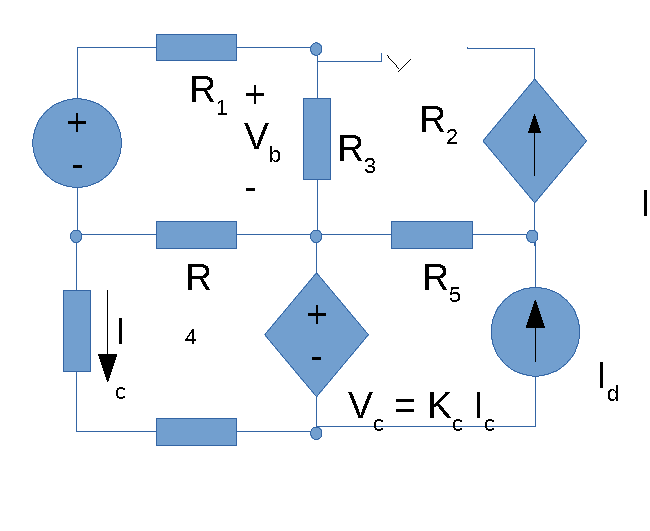
\includegraphics[width=10 cm]{rc.pdf}
\caption{Given circuit}
\label{fig:circuit}
\end{figure}
